\begin{tikzpicture}[scale=0.5,remember picture]
    \begin{scope}
    \begin{pgfinterruptboundingbox}
        \draw [rotate=-10, clip]  (4.1,2.8) rectangle (5.6,-0.2)[reverseclip];
        \draw [rotate=30, clip] (0.5,1.4) rectangle (2,-1.6)[reverseclip];
        \draw [rotate=10, clip] (3.5,-3.8) rectangle (5,-6.8)[reverseclip];
        \draw [rotate=-10, clip] (10.5,4.2) rectangle (12,1.2)[reverseclip];
        \draw [rotate=15, clip] (9.3,-6.2) rectangle (10.8,-9.2)[reverseclip];
        \draw [rotate=91, clip] (-3,-6.6) rectangle (-1.5,-9.6)[reverseclip];
        \draw [rotate=-20, clip] (2.1,-2.2) rectangle (3.6,-5.2)[reverseclip];
        \end{pgfinterruptboundingbox}
        \draw [blue] plot[smooth, tension=.7] coordinates {(-8,-2) (-4,-1) (-1,0) (3,1) (8,1) (13,1) (15,1)};
        \draw [blue] plot[smooth, tension=.7] coordinates {(-8,-3) (-3,-3) (0.8,-4.6) (7,-5) (14,-5) (15,-5)};
        \draw [blue] plot[smooth, tension=.7] coordinates {(-2,-2) (0,-1) (3,0) (7,-1) (7,-3) (4,-4) (-1,-3) (-2,-2)};
        \draw [blue] plot[smooth, tension=.7] coordinates {(15,0) (10,0) (9,-2) (10,-4) (14,-4) (15,-4)};
    \end{scope}

    \draw [thick, green]  plot[smooth, tension=.7] coordinates {(5.2,4.2) (0.8,3.4) (0.4,1.2) (1.8,-0.6) (3.2,-2) (4.8,-2.6) (5.4,-4.6) (5,-8.4)};
    \draw [thick, green]  plot[smooth, tension=.7] coordinates {(5.2,4.2) (4.8,2.6) (5,1) (4.4,-1.2) (3.2,-2) (1.8,-2.6) (1.2,-4.2) (0.8,-6.4) (3,-7.6) (5,-8.4)};
    \draw [thick, green]  plot[smooth, tension=.7] coordinates {(5.2,4.2) (10.6,3.2) (11.8,2) (11.4,-0.4) (11.2,-2.4) (11.6,-3.8) (12,-7.2) (7.4,-7.8) (5,-8.4)};
    \draw [thick, green]  plot[smooth, tension=.7] coordinates {(3.2,-2) (5,-2) (8,-1.8) (10.2,-2.4) (11.2,-2.4)};

    \node [green] at (3.2,-2) [circle] {$\bullet$};
    \node [green]at (11.2,-2.4) [circle] {$\bullet$};
    \node [green]at (5,-8.4) [circle] {$\bullet$};
    \node [green]at (5.2,4.2) [circle] {$\bullet$};
\end{tikzpicture}

\paragraph{Definition} \parskp
Ein Graph ist ein Paar $V,E$ mit $V\ne\emptyset$ und $E$ ist eine zweielementige Menge von $V$. $V$ ist die
Menge der Knoten. $E$ die Menge der Kanten.

\paragraph{Beispiel} \parskp
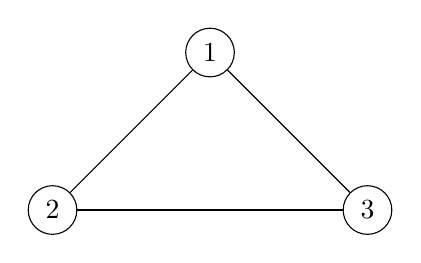
\begin{tikzpicture}
    \node[shape=circle,draw=black] (1) at (0,0)   {1};
    \node[shape=circle,draw=black] (2) at (-2,-2) {2};
    \node[shape=circle,draw=black] (3) at (2,-2)  {3};

    \path (1) edge (2);
    \path (2) edge (3);
    \path (3) edge (1);
\end{tikzpicture}\\
Graph $G=(\{1,2,3\},\{1,2\},\{2,3\},\{3,1\})$\\
\\
\begin{tikzpicture}
    \node[shape=circle,draw=black] (1) at (0,0)  {1};
    \node[shape=circle,draw=black] (2) at (4,0)  {2};
    \node[shape=circle,draw=black] (3) at (2,-2) {3};

    \path (1) edge (2);
\end{tikzpicture}\\
Graph $H=(\{1,2,3\},\{1,2\})$

\paragraph{Definition} \parskp
Ein Graph hei"st vollst"andig, wenn alle Knoten paarweise miteinander verbunden sind.
\subparagraph{Folgerung} Ein vollst"andiger Graph mit $n$ Knoten besitzt $\binom{n}{2}$ Kanten.

\paragraph{Definition}  \parskp
Ein Knoten $v$ besitzt den Grad $k$, wenn er mit genau $k$ Kanten verbunden ist.
\subparagraph{Notation} $deg(v)=k$

\paragraph{Satz} F"ur jeden Graphen $(V,E)$ gilt
\begin{align*}
    \sum{v\in V}deg=2|E|
\end{align*}

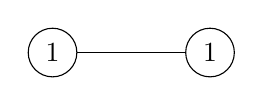
\begin{tikzpicture}
    \node[shape=circle,draw=black] (1) at (0,0) {1};
    \node[shape=circle,draw=black] (2) at (2,0) {1};

    \path (1) edge (2);
\end{tikzpicture}
$|E|=1$\qquad
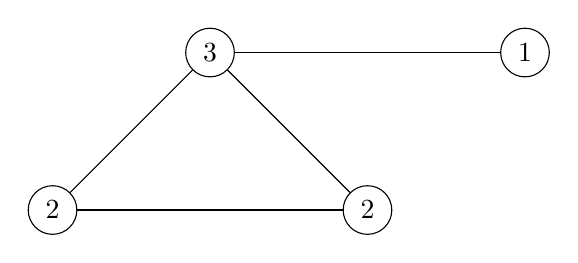
\begin{tikzpicture}
    \node[shape=circle,draw=black] (1) at (0,0) {2};
    \node[shape=circle,draw=black] (2) at (2,2) {3};
    \node[shape=circle,draw=black] (3) at (4,0) {2};
    \node[shape=circle,draw=black] (4) at (6,2) {1};

    \path (1) edge (2);
    \path (2) edge (3);
    \path (3) edge (1);
    \path (2) edge (4);
\end{tikzpicture}
$|E|=4$

\paragraph{Beweis} \parskp
Wenn wir jede Kante in der Mitte durchschneiden, ist jeder Knoten $V$ mit genau $deg(v)$ H"alften verbunden.
Die Summe aller Knotengrade ist dann die Anzahl der Knotenh"alften.

\paragraph{Definition}
\begin{itemize}
    \item Ein \textbf{Weg} ist eine Folge von Knoten $v_0,\cdots,v_l$ mit $\{v_k,v_{k+1}\}$ f"ur $1\le k<l$.\\
          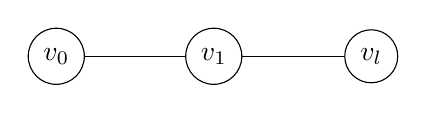
\begin{tikzpicture}
              \node[shape=circle,draw=black] (1) at (0,0) {$v_0$};
              \node[shape=circle,draw=black] (2) at (2,0) {$v_1$};
              \node[shape=circle,draw=black] (3) at (4,0) {$v_l$};

              \path (1) edge (2);
              \path (2) edge (3);
          \end{tikzpicture}
    \item Ein Graph ist \textbf{zusammenh"angend}, wenn es f"ur alle Knoten $u,v$, $u\ne v$ einen Weg von $u$
          nach $v$ gibt.
    \item Ein \textbf{Pfad} ist ein Weg, der keine Knoten mehrfach enth"alt.
    \item Ein \textbf{Kreis} ist ein Weg, $v_0,\cdots,v_l$ mit $v_0=v_l$, der keinen Knoten mehrfach enth"alt
          bis auf Startknoten und Endknoten und eine L"ange $\ge3$ beitzt.
\end{itemize}

\section{B"aume}

\paragraph{Definition} \parskp
Ein \textbf{Baum} ist ein zusammenh"angender Graph, der keinen Kreis enth"alt.\\
\\
Ein Blatt ist ein Knoten mit dem Grad $\le1$\\
\begin{tikzpicture}[level distance=1.5cm,
    level 2/.style={sibling distance=3cm},
    level 3/.style={sibling distance=1.5cm}]
    \node[shape=circle,draw=black] {}
      child {node[shape=circle,draw=black] {}
        child {node[shape=circle,draw=black] {}
          child {node[shape=circle,draw=black] {}}
          child {node[shape=circle,draw=black] {}}
        }
        child {node[shape=circle,draw=black] {}
          child {node[shape=circle,draw=black] {}}
          child {node[shape=circle,draw=black] {}}
        }
      };
\end{tikzpicture}\hspace{2.5cm}
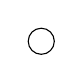
\begin{tikzpicture}
    \node[shape=circle,draw=black] {};
\end{tikzpicture} \qquad \tgrey{Ist auch ein Baum}

\paragraph{Lemma} Jeder Baum enth"alt ein Blatt.

\paragraph{Satz} Sei $B=(V,E)$ ein Baum. \\
Dann gilt $|E|=|V|-1$.\\
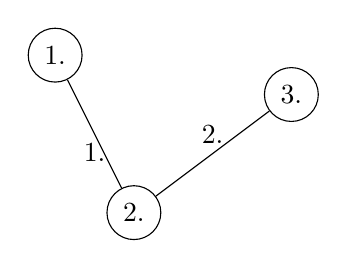
\begin{tikzpicture}
    \node[shape=circle,draw=black] (1) at (0,2)   {1.};
    \node[shape=circle,draw=black] (2) at (1,0)   {2.};
    \node[shape=circle,draw=black] (3) at (3,1.5) {3.};

    \path (1) edge node[below] {1.} (2);
    \path (2) edge node[above] {2.} (3);
\end{tikzpicture}\qquad \tgrey{Es gibt nur einen Knoten, dem keine Kante hinzugef"ugt wird.}

\paragraph{Beweis} Induktion nach der Anzahl der Knoten $n$
\begin{itemize}
    \item[$n=1$] Ein Baum mit einem Knoten enth"alt keine Kanten.
    \item[$n\rightarrow n+1$] Sei $B$ ein Baum mit $n+1$ Knoten. Da $B$ ein Baum ist, enth"alt $B$ ein Blatt.
                              Indem wir dieses Blatt und die dazugeh"orige Kante entfernen, erhalten wir einen
                              Baum $B'$ mit $n$ Knoten. Nach Induktionsvoraussetzung folgt:\\
                              $B'$ enth"alt $n-1$ Knoten. Indem wir die oben entfernten Knoten mit samt der mit
                              ihm verbundenene Kante hinzuf"ugen, erhalten wie den Baum $B$. Dieser besitzt $n+1$
                              Knoten und $n$ Kanten.
\end{itemize}

\paragraph{Definition} \parskp
Ein \textbf{bin"arer Wurzelbaum} ist ein Baum, der eine Knoten-Wurzel besitzt und in dem jeder Knoten, der
kein Blatt ist genau zwei Nachfolger besitzt.\\
\\
Dazu gleichwertig ist die folgende \underline{induktive Definition}.
\begin{itemize}
    \item Ein Knoten $v$ ist ein bin"arer Wurzelbaum mit Wurzel $v$.
    \item Seien $l,r$ bin"are Wurzelb"aume mit den Wurzeln $root(l)$, $root(r)$. Wenn wir einen neune
          Knoten $v$ mit $root(l)$, $root(r)$ verbinden, ist das Ergebnis ein bin"arer Wurzelbaum mit
          Wurzel $v$.
\end{itemize}

\paragraph{Satz} \parskp
Sei $B$ ein bin"arer Wurzelbaum, in dem jeder Pfad von der Wurzel zu einem Blatt der L"ange $k$ hat
($B$ besitzt die L"ange $k$), dann besitzt $B$ genau $2^k$ Bl"atter.

\subparagraph{Beweis} Induktion nach $k$.
\begin{itemize}
    \item[$k:=0$] In diesem Fall besteht $B$ nur aus der Wurzel und besitzt $2^0=1$ Bl"atter.
    \item[$k\rightarrow k+1$] Sei $B$ ein Baum der Tiefe $k+1$. Jeder der beiden Teilb"aum unter der Wurzel
                            ist ein bin"arer Wurzelbaum der Tiefe $k$. Nach Induktionsvoraussetzung besitzt
                            jeder dieser Teilb"aume genau $2^k$ Bl"atter. Folglich besitzt $B$ genau
                            $2^{k+1}$ Bl"atter.
\end{itemize}

\newpage
\section{Datenstrukturen zur Representation}

Zur Darstellung von Graphen werden \textbf{Adjazenzmatrizen} und \textbf{Adjazenzlisten} verwendet.

\paragraph{Definition} Sei $G=(V,E)$ ein Graph
\begin{itemize}
    \item Die Adjazenzmatrix $G$ ist eine Matrix $(a_{uv})$ mit
          \[
            a_{uv}=\begin{cases}
                1 & \for \{u,v\}\in E\\
                0 & \text{sonst}
            \end{cases}
          \]
    \item Die Adjazenzliste von $G$ ist ein Feld, dass an der Position $u\in V$ eine Liste aller Knoten
          $v\in V$ mit $\{u,v\}\in E$ besitzt.
\end{itemize}
Der Speicherbedarf der Adjazenzmatrix liegt in $O(|V|^2)$, der der Adjazenzliste in $O(|V|+|E|)$. Bei
Graphen mit wenig Kanten ist die Adjazenzliste im Vorteil.\parskp
\\
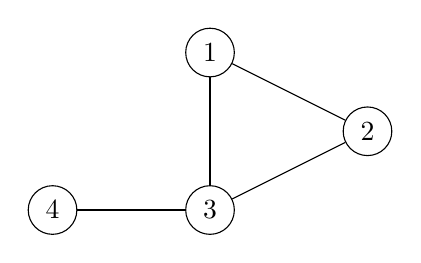
\begin{tikzpicture}
    \node[shape=circle,draw=black] (4) at (0,0) {4};
    \node[shape=circle,draw=black] (1) at (2,2) {1};
    \node[shape=circle,draw=black] (3) at (2,0) {3};
    \node[shape=circle,draw=black] (2) at (4,1) {2};

    \path (4) edge (3);
    \path (3) edge (1);
    \path (1) edge (2);
    \path (2) edge (3);
\end{tikzpicture}\\
\[
    \begin{pmatrix}
        0 & 1 & 1 & 0 \\
        1 & 0 & 1 & 0 \\
        1 & 1 & 0 & 1 \\
        0 & 0 & 1 & 0
    \end{pmatrix}
\]
\begin{align*}
    \fbox{1} & \rightarrow\fbox{2}\fbox{3} \\
    \fbox{2} & \rightarrow\fbox{2}\fbox{3} \\
    \fbox{3} & \rightarrow\fbox{1}\fbox{2}\fbox{4} \\
    \fbox{4} & \rightarrow\fbox{3}
\end{align*}\\
Wurzelb"aume lassen sich durch rekursive Datenstrukturen darstellen. Jeder Knoten enth"alt dabei eine Liste
der Nachfolgeknoten. Ein bin"arer Wurzelbaum l"asst sich darstellen durch Knotenelemente, die Zeiger links
und rechts, f"ur den linken bzw. rechten Nachfolger besitzt.

\paragraph{Beisiel} Implementierung in C
\begin{lstlisting}[language=C]
struct bintree {
    int value;
    struct bintree *left, *right;
}
\end{lstlisting}

\section{Grundlegende Graphenalgorithmen}
\subsection{Breitensuche und Tiefensuche}

\textbf{Breitensuche} und \textbf{Tiefensuche} sind Algorithmen, um Knoten eines Graphen systematisch zu
durchsuchen. Die Breitensuche besucht, ausgehend von dem Startknoten, alle Nachbarn eines Knoten und dessen
Nachbarn, bis der Zielknoten gefunden wurde.

\paragraph{Breitensuche}
\subparagraph{Beispiel} Breitensuche in einem Wurzelbaum\\
\begin{tikzpicture}[level distance=1.5cm,
    level 1/.style={sibling distance=3cm},
    level 2/.style={sibling distance=1.5cm}]
    \node {0}
      child {node {1}
        child {node {4}
          child {node {8}}
          child {node {9}}
          child {node {10}}
        }
      }
      child {node {2}
        child {node {5}}
        child {node {6}}
      }
      child {node {3}
        child {node {7} 
          child {node {11}}
        }
      };
\end{tikzpicture}
\\
Eine Breitensuche kann mit einer \textbf{Queue} implementiert werden. Eine Queue ist eine
\textit{first in first out} (FIFO) Datenstruktur die zwei Operationen besitzt.
\begin{itemize}
    \item \code{v=dequeue()}
    \item \code{enqueue(v)}
\end{itemize}
Eine Queue l"asst sich effizient implementieren, durch eine verkettete Liste, die einen Zeiger auf das n"achste
Element besitzt. Damit lassen sich \code{dequeue} und \code{enqueue} in Zeit $O(1)$ ausf"uhren.

\subparagraph{Algorithmus} Breitensuche (breadth first search)
\begin{lstlisting}[language=C]
boolean bfs(node start, node end) {
    for (v of V)
        discovered[v] = false
    queue.enqueue(start)
    discovered[start] = true
    while (!queue.isEmpty()) {
        u = queue.dequeue()
        if (u = end) return true
        else
            for (v of adj[v])
                if (!discovered[v]) {
                    queue.enqueue(v)
                    discovered[v] = true
                }
    }
    return false
}
\end{lstlisting}

\subparagraph{Analyse der Lafzeit} \parskp
Das Initialisieren des Felds \code{discovered} ben"otigt die Zeit $O(|V|)$. Im Rumpf der \code{while} Schleife
f"allt der Aufwand $O(deg(u))$ an. Der Gesamtaufwand der \code{while} Schleife ist
\[
    \sum{u\in V}O(deg(u))\le c\sum{u\in V}deg(u)=c2|E|\in O(|E|)
\]
Der Aufwand insgesamt ist daher $O(|V|+|E|)$.

\paragraph{Tiefensuche} \parskp
Die Tiefensuche verfolgt den Pfad, bis ein Knoten keine unbesuchten Nachbarn mehr besitzt.

\subparagraph{Beispiel} Tiefensuche in einem Wurzelbaum\\
\begin{tikzpicture}[level distance=1.5cm,
    level 1/.style={sibling distance=3cm},
    level 2/.style={sibling distance=1.5cm}]
    \node {0}
      child {node {1}
        child {node {2}
          child {node {3} {
            child {node {4}}
            child {node {5}}
          }}
        }
        child {node {6}}
      }
      child {node {7}}
      child {node {8}
        child {node {9} {
          child {node {10} {
            child {node {11}}
            child {node {12}}
          }}
        }}
        child {node {13}}
      };
\end{tikzpicture}

\subparagraph{Implementierung} Tiefensuche (depth first search)
\begin{enumerate}
    \item Gleicher Algorithmus wie Breitensuche aber mit \textbf{Stack} statt Queue. Ein Stack ist ein
          \textit{last in first out} (LIFO) Datentyp, der sich durch eine verkettete Liste implementieren
          l"asst und zwei Operationen besitzt \code{push} und \code{pop}.
    \item Rekursiv. In jedem Nachbarknoten wird eine neue Tiefensuche gestartet.
          \begin{lstlisting}[language=C]
          dfs(Graph G, node v) {
              u.visited = true
              for (v in G.adj[v])
                if (v.visited == false) dfs(G, v)
          }

          init(Graph G, node v) {
              for (v in G) {
                u.visited = false
                for (v in G)
                  dfs(G, v)
              }  
          }
          \end{lstlisting}
\end{enumerate}

\paragraph{Definition} Sei $G=(V,E)$ ein \textbf{DAG} (directed acyclic graph, gerichteter azyklischer Graph)\\
Eine \textbf{topologische Sortierung} von $G$ ist eine Abbildung $f:V\rightarrow\NN$ mit $f(u)>f(v)$ f"ur $(u,v)\in E$.
\\
\lecdate{26.11.2018}
\\
Eine topologische Sortierung kann durch eine Tiefensuche bestimmt werden.
\begin{lstlisting}
    topsort:
        for (v in V)
            markiere v mit weiß
        for (v in V)
            tiefensuche(v)

    tiefensuche(v)
        v grau: Fehler, da Graph einen Kreis enthält
        v weiß: markiere v mit grau
            for {u|(v,u) in E}
                tiefensuche(u)
            markiere v mit schwarz und füge v an den Kopf der sortierten Liste an
\end{lstlisting}

\section{Suche}
\subsection{Lineare Suche}

Laufzeit \(O(n)\), daher ung"unstig bei gro"sen \(n\)

\subsection{Bin"are Suche}

Voraussetzung f"ur eine \textbf{bin"are Suche} ist ein sortiertes Array.

\paragraph{Idee des Algorithmus}
Das gesuchte Element wird mit dem Element in der Mitte des Arrays verglichen. Ist es kleiner, wird in der linken H"alfte des Arrays weitergesucht,
sont in der rechten H"alfte. Das Verfahren wird beendet, wenn das Element gefunden wurde oder die H"alften die L"ange 0 beistzten.

\paragraph{Beispiel} Suche nach \(8\) in \(\{1,3,4,5,6,10,11,15,16,22,30\}\)\\
\begin{tabular}{ m{11cm} m{5cm} }
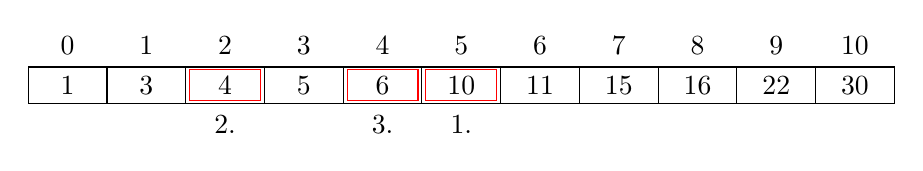
\begin{tikzpicture}
    \foreach \x in {0,...,10} {
        \node at (\x, 0) {\tred{\x}};
    }
    \node (0) [draw, minimum width=1cm] at (0, -0.5) {1};
    \node (1) [draw, minimum width=1cm] at (1, -0.5) {3};
    \node (2) [draw, minimum width=1cm] at (2, -0.5) {4};
    \node (3) [draw, minimum width=1cm] at (3, -0.5) {5};
    \node (4) [draw, minimum width=1cm] at (4, -0.5) {6};
    \node (5) [draw, minimum width=1cm] at (5, -0.5) {10};
    \node (6) [draw, minimum width=1cm] at (6, -0.5) {11};
    \node (7) [draw, minimum width=1cm] at (7, -0.5) {15};
    \node (8) [draw, minimum width=1cm] at (8, -0.5) {16};
    \node (9) [draw, minimum width=1cm] at (9, -0.5) {22};
    \node (10) [draw, minimum width=1cm] at (10, -0.5) {30};

    \node (2r) [draw=red, minimum width=0.9cm, minimum height=0.4cm] at (2, -0.5) {};
    \node (4r) [draw=red, minimum width=0.9cm, minimum height=0.4cm] at (4, -0.5) {};
    \node (5r) [draw=red, minimum width=0.9cm, minimum height=0.4cm] at (5, -0.5) {};

    \node (2n) at (2, -1) {\tred{2.}};
    \node (4n) at (4, -1) {\tred{3.}};
    \node (5n) at (5, -1) {\tred{1.}};
\end{tikzpicture} &
8 konnte nicht gefunden werden.
\end{tabular}

\rule{\textwidth}{0.2pt}
\\
\\
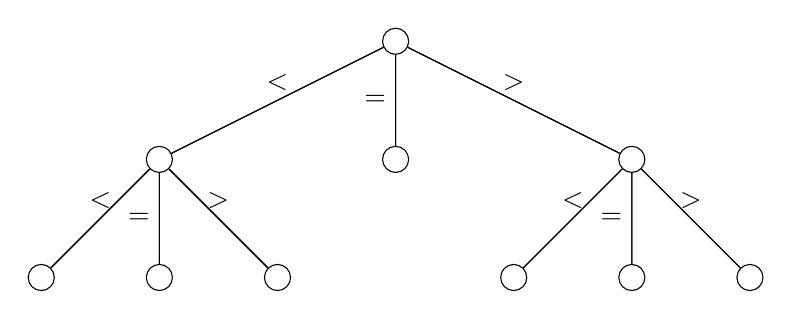
\begin{tikzpicture}[level distance=1.5cm,
    level 1/.style={sibling distance=3cm},
    level 2/.style={sibling distance=1.5cm}]
    \begin{scope}[every node/.style={draw, circle, thin}]
    \node (0) {}
    child {node (1) {}
      child {node (2) {}}
      child {node (3) {}}
      child {node (4) {}}
    }
    child {node (5) {}}
    child {node (6) {}
      child {node (7) {}}
      child {node (8) {}}
      child {node (9) {}}
    };
    \end{scope}

    \path (0) edge node[above] {\(<\)} (1);
    \path (1) edge node[above] {\(<\)} (2);
    \path (1) edge node[left] {\(=\)} (3);
    \path (1) edge node[above] {\(>\)} (4);
    \path (0) edge node[left] {\(=\)} (5);
    \path (0) edge node[above] {\(>\)} (6);
    \path (6) edge node[above] {\(<\)} (7);
    \path (6) edge node[left] {\(=\)} (8);
    \path (6) edge node[above] {\(>\)} (9);
\end{tikzpicture}\qquad
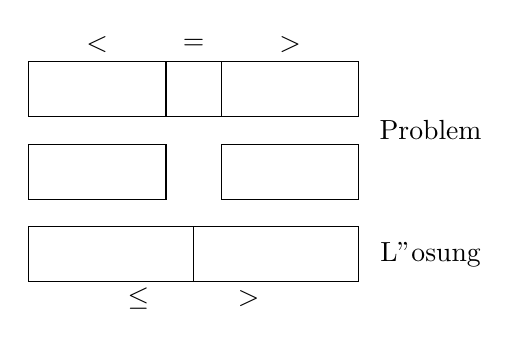
\begin{tikzpicture}[scale=0.7]
    \draw (0,0) rectangle (6,1);
    \draw (3,0) -- (3,1);
    \node at (2,-0.3) {\(\le\)};
    \node at (4,-0.3) {\(>\)};

    \draw (0,1.5) rectangle (2.5,2.5);
    \draw (3.5,1.5) rectangle (6,2.5);
    \node at (7.3,2.75) {Problem};

    \node at (1.25,4.3) {\(<\)};
    \node at (3,4.3) {\(=\)};
    \node at (4.75,4.3) {\(>\)};
    \draw (0,3) rectangle (6,4);
    \draw (2.5,3) -- (2.5,4);
    \draw (3.5,3) -- (3.5,4);
    \node at (7.3,0.5) {L"osung};
\end{tikzpicture}

\paragraph{Laufzeitanalyse} \parskp
Wir vereinfachen dazu den Algorithmus so, dass nur Vergleiche mit \(\le\) und \(>\) ausgef"uhrt werden und das Array stets halbiert wird. Ferner
nehmen wir an, dass die L"ange des Arrays \(2^k\) ist. Dann l"asst sich das Verhlaten der bin"aren Suche im Worst-Case (Element nicht vorhanden)
als vollst"andiger Bin"arbaum darstellen.\\
\begin{tabular}{ m{8cm} m{8cm} }
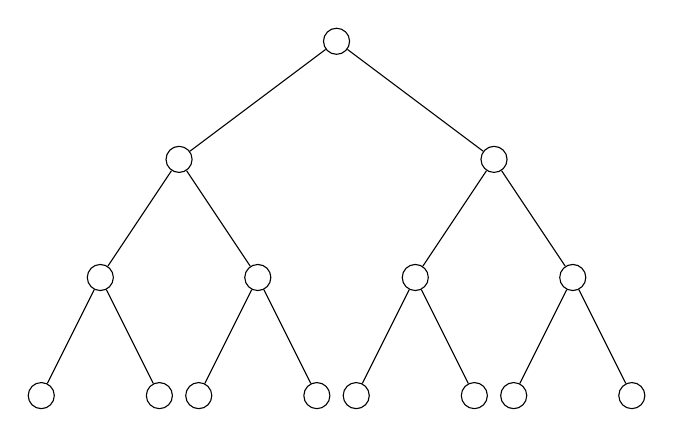
\begin{tikzpicture}[level distance=1.5cm,
    level 1/.style={sibling distance=4cm},
    level 2/.style={sibling distance=2cm},
    level 3/.style={sibling distance=1.5cm}]
    \node[shape=circle,draw=black] {}
    child {node[shape=circle,draw=black] {}
      child {node[shape=circle,draw=black] {}
        child {node[shape=circle,draw=black] {}}
        child {node[shape=circle,draw=black] {}}}
      child {node[shape=circle,draw=black] {}
        child {node[shape=circle,draw=black] {}}
        child {node[shape=circle,draw=black] {}}
      }
    }
    child {node[shape=circle,draw=black] {}
      child {node[shape=circle,draw=black] {}
        child {node[shape=circle,draw=black] {}}
        child {node[shape=circle,draw=black] {}}}
      child {node[shape=circle,draw=black] {}
        child {node[shape=circle,draw=black] {}}
        child {node[shape=circle,draw=black] {}}
      }
    };
\end{tikzpicture} &
Jedes Blatt entspricht einem Vergliech mit \(n\)-Feldelementen. Der Baum besitzt daher die Tefe \(k=\log n\).
\end{tabular}\\
\\
\\
Die Laufzeit der bin"aren Suche liegt daher in \(O(\log n)\).

\subsection{Binäre Suchbäume}
\lecdate{03.12.2018}
Ein Suchbaum ist ein bin"arer Wurzelbaum, in dem gilt, dass jeder in einem Knoten gespeicherter Wert gr"o"ser ist,
als alle Knoten in seinem linken Teilbaum und kleiner ist, als alle Knoten in seinem rechten Teilbaum.

\paragraph{Beispiel} \parskp
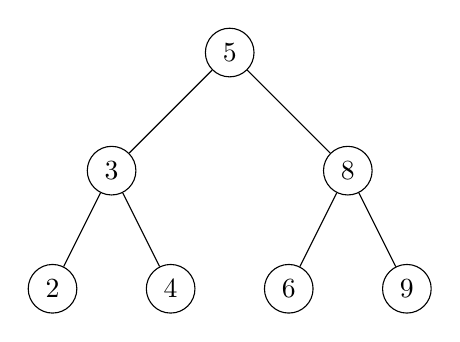
\begin{tikzpicture}[level distance=1.5cm,
    level 1/.style={sibling distance=3cm},
    level 2/.style={sibling distance=1.5cm},
    every node/.style={draw, circle, thin}]
    \node {5}
      child {node {3}
        child {node {2}}
        child {node {4}}
      }
      child {node {8}
        child {node {6}}
        child {node {9}}
      };
\end{tikzpicture}
